\documentclass[10pt]{article}

\usepackage{pictex, latexsym, graphicx,amsmath,amssymb,amsbsy,amsfonts,amsthm,verbatim}
\usepackage{fullpage}
\usepackage{graphics}
\usepackage{fancyhdr}

\usepackage{algorithm,algorithmic}
\usepackage{multirow}
\usepackage{tikz}
\usepackage{xcolor}

\setlength{\voffset}{-0.25in}
\setlength{\headsep}{0.25in}
\setlength{\parskip}{1em}
\setlength{\parindent}{0em}

\newcounter{problem}
\newcommand{\problem}{\textbf{\refstepcounter{problem}Problem \theproblem.} }


\def\vu{\mathbf{u}}
\def\vx{\mathbf{x}}
\def\vb{\mathbf{b}}
\def\vv{\mathbf{v}}
\def\vw{\mathbf{w}}

\renewcommand{\implies}{\rightarrow}
\renewcommand{\lor}{\vee}
\renewcommand{\land}{\wedge}
\newcommand{\xor}{\oplus}
\renewcommand{\iff}{\leftrightarrow}
\newcommand{\TRUE}{\mathbf{T}}
\newcommand{\FALSE}{\mathbf{F}}
\newcommand{\universe}{\mathcal{U}}

\begin{document}
\pagestyle{fancyplain}
\title{Chapter 8: Introduction to graph}

	\textbf{Exercise 4.} \\
For each course at a university, there may be one or more other courses that are its prerequisites. How can a graph be used to model these courses and which courses are prerequisites for which courses? Should edges be directed or undirected? Looking at the graph model, how can we find courses that do not have any prerequisites and how can we find courses that are not the prerequisite for any other courses\\
Answer:\\
We use a directed graph, with an edge $(u,v)$ defines the subject $"u"$ is a prerequisites for subject $"v"$.\\
When the subject doesn't have any prerequisites, it has no in-degree. When the subject is not the prerequisite for any other courses, it has no out-degree or out-degree equals 0.\\

	\textbf{Exercise 5.}\\
Find the number of vertices, the number of edges, and the degree of each vertex in the given undirected graph. Identify all isolated and pendant vertices.\\
Answer:\\
+Graph 1:\\
\begin{tikzpicture}
	\filldraw [black]
			(0,0) circle (2pt) node[below] {f}
			(2,0) circle (2pt) node[below] {e}
			(0,2) circle (2pt) node[above] {a}
			(2,2) circle (2pt) node[above] {b}
			(4,2) circle (2pt) node[above] {c}
			(4,0) circle (2pt) node[below] {d};
	\draw (4,2) -- (2,2) -- (0,2) -- (0,0) -- (2,2) -- (2,0) -- (0,0);
	\end{tikzpicture}
	\bigbreak
The number of vertices: 6 - edges: 6 - isolated vertices: d - pendant vertices: c.\\
The degree of each vertex:\\
a : 2 - b : 4 - c : 1 - d : 0 - e : 2 - f : 3\\
+Graph 2:\\
\begin{tikzpicture}[node distance=2cm]
	\tikzstyle{edge} = [draw=black, line width=2]
	\filldraw [black]
			(0,0) circle (3pt)
			(0,2) circle (3pt)
			(2,2) circle (3pt)
			(2,0) circle (3pt)
			(4,0) circle (3pt);
		\node[] (a) at (0,2)  [label=above:$a$] {};
        \node[] (b) at (2,2)  [label=above:$b$] {};
		\node[] (e) at (0,0)  [label=below:$e$] {};
		\node[] (d) at (2,0)  [label=below:$d$] {};
		\node[] (c) at (4,0)  [label=below:$c$] {};

		\draw (b) -- (a) -- (e) -- (d) -- (b) -- (e);
		\draw (d) -- (c) -- (b);
		\path
		(a) edge[bend right] node {} (b)
		(a) edge[bend left] node {} (b);
		\path 
		(a) edge[loop left] node {} (a);
		\path
		(c) edge[loop right] node {} (c);
	\end{tikzpicture}
	\bigbreak
 number of vertices: 5 - edges: 13 - isolated vertices: none - pendant vertices: none.\\
The degree of each vertex:\\
a : 6 - b : 6 - c : 6 - d : 5 - e : 3\\
+Graph 3:\\
\bigbreak
	\begin{tikzpicture}[node distance=2cm]
	\tikzstyle{edge} = [draw=black, line width=2]
	\filldraw [black]
			(0,0) circle (3pt)
			(2,0) circle (3pt)
			(2,2) circle (3pt)
			(4,2) circle (3pt)
			(4,0) circle (3pt)
			(6,2) circle (3pt)
			(6,0) circle (3pt)
			(8,2) circle (3pt)
			(8,0) circle (3pt); 
		\node[] (a) at (2,2)  [label=above:$a$] {};
        \node[] (b) at (4,2)  [label=above:$b$] {};
		\node[] (c) at (6,2)  [label=above:$c$] {};
		\node[] (d) at (8,2)  [label=below:$d$] {};
		\node[] (e) at (8,0)  [label=below:$e$] {};
		\node[] (g) at (6,0)  [label=below:$g$] {};
		\node[] (h) at (4,0)  [label=below:$h$] {};
		\node[] (i) at (2,0)  [label=below:$i$] {};
		\node[] (f) at (0,0)  [label=below:$f$] {};

		\draw (a) -- (i) -- (h) -- (b) -- (e) -- (c) -- (g);
		\draw (a) -- (e);
		\draw (b) -- (e);
		\draw (i) -- (c);
		\path (g) edge [bend left] node{} (e)
			  (g) edge [bend right] node{} (e)
			  (a) edge [bend left] node{} (c);
	\end{tikzpicture}
\bigbreak
The number of vertices: 9 - edges: 12 - isolated vertices: 2 - pendant vertices: none.\\
The degree of each vertex:\\
a : 3 - b : 2 - c : 4 - d : 0 - e : 6 - f : 0 - g : 4 - h : 2 - i : 3\\

	\textbf{Exercise 6.}\\
Can a simple graph exist with 15 vertices each of degree five?\\
Answer:\\
We have 15 vertices of $deg(5) \implies$ the total sum of all degree equals 75 $\implies$ wrong.\\

	\textbf{Exercise 7.}\\
Determine the number of vertices and edges and find the in-degree and out-degree of each vertex for the given directed multigraph.\\
Answer:\\ 
* vertice has the in-degree of x $\implies$ vertice: x in\\
\large(+Graph 1:)\\
We have 4 vertices and 7 edges.\\
Vertice a: 1 out, 3 in.\\
Vertice b: 2 out, 1 in.\\
Vertice c: 1 out, 2 in.\\
Vertice d: 3 out, 1 in.\\
\large(+Graph 2:)\\
We have 4 vertices and 8 edges.\\
Vertice a: 2 out, 2 in.\\
Vertice b: 4 out, 3 in.\\
Vertice c: 1 out, 2 in.\\
Vertice d: 1 out, 1 in.\\
\large(+Graph 3:)\\
We have 5 vertices and 13 edges.\\
Vertice a: 1 out, 6 in.\\
Vertice b: 5 out, 1 in.\\
Vertice c: 5 out, 2 in.\\
Vertice d: 4 out, 2 in.\\
Vertice e: 0 out, 0 in.\\

	\textbf{Exercise 8:}\\
Draw these graphs\\
a) $\textit{$K_{7}$}$\\
b) $\textit{$K_{1,8}$}$\\
c) $\textit{$K_{4,4}$}$\\
d) $\textit{$C_{7}$}$\\
e) $\textit{$W_{7}$}$\\
f) $\textit{$Q_{4}$}$\\
\underline{Answer:}\\
\begin{itemize}
	\item $K_7$\\
	\bigbreak
	\begin{tikzpicture}[node distance=2cm]
	\tikzstyle{edge} = [draw=black, line width=2]
	\filldraw [black]
			(0,0) circle (3pt)
			(0,-2) circle (3pt)
			(2,2) circle (3pt)
			(4,2) circle (3pt)
			(6,0) circle (3pt)
			(6,-2) circle (3pt)
			(3,-4) circle (3pt);
		\node[] (b) at (0,0)  [label=left:$b$] {};
        \node[] (a) at (0,-2) [label=above:$a$] {};
		\node[] (c) at (2,2)  [label=above:$c$] {};
		\node[] (d) at (4,2)  [label=above:$d$] {};
		\node[] (e) at (6,0)  [label=right:$e$] {};
		\node[] (f) at (6,-2) [label=right:$f$] {};
		\node[] (g) at (3,-4) [label=below:$g$] {};
	\draw (a) -- (b) -- (c) -- (d) -- (e) -- (f) -- (g);
	\draw (a) -- (c);
	\draw (a) -- (e);
	\draw (a) -- (f);
	\draw (a) -- (g);
	\draw (b) -- (d);
	\draw (b) -- (e);
	\draw (b) -- (f);
	\draw (b) -- (g);
	\draw (c) -- (e);
	\draw (c) -- (f);
	\draw (c) -- (g);
	\draw (d) -- (f);
	\draw (d) -- (g);
	\draw (e) -- (g);
	\end{tikzpicture}
	\item $K_{1,8}$ \\
	\bigbreak
    \begin{tikzpicture}[node distance=2cm]
	\tikzstyle{edge} = [draw=black, line width=1]
	\filldraw [black]
			(0,0) circle (3pt)
			(1,0) circle (3pt)
			(2,0) circle (3pt)
			(3,0) circle (3pt)
			(4,0) circle (3pt)
			(5,0) circle (3pt)
			(6,0) circle (3pt)
			(7,0) circle (3pt)
			(3,3) circle (3pt);
		\node[] (a) at (0,0)  [label=below:$a$] {};
        \node[] (b) at (1,0)  [label=below:$b$] {};
		\node[] (c) at (2,0)  [label=below:$c$] {};
		\node[] (d) at (3,0)  [label=below:$d$] {};
		\node[] (e) at (4,0)  [label=below:$e$] {};
		\node[] (f) at (5,0)  [label=below:$f$] {};
		\node[] (g) at (6,0)  [label=below:$g$] {};
		\node[] (h) at (7,0)  [label=below:$h$] {};
		\node[] (i) at (3,3)  [label=above:$i$] {};
  	\draw (i) -- (a);
  	\draw (i) -- (b);
  	\draw (i) -- (c);
  	\draw (i) -- (d);
  	\draw (i) -- (e);
  	\draw (i) -- (f);
  	\draw (i) -- (g);
  	\draw (i) -- (h);
	\end{tikzpicture}
	\item $K_{4,4}$\\
	\bigbreak
	\begin{tikzpicture}[node distance=2cm]
	\tikzstyle{edge} = [draw=black, line width=1]
	\filldraw [black]
            (0,0) circle (3pt)
			(2,0) circle (3pt)
			(4,0) circle (3pt)
			(6,0) circle (3pt)
			(0,2) circle (3pt)
			(2,2) circle (3pt)
			(4,2) circle (3pt)
			(6,2) circle (3pt);
		\node[] (h) at (0,0)  [label=below:$h$] {};
        \node[] (g) at (2,0)  [label=below:$g$] {};
		\node[] (f) at (4,0)  [label=below:$f$] {};
		\node[] (e) at (6,0)  [label=below:$e$] {};
		\node[] (d) at (6,2)  [label=above:$d$] {};
		\node[] (c) at (4,2)  [label=above:$c$] {};
		\node[] (b) at (2,2)  [label=above:$b$] {};
		\node[] (a) at (0,2)  [label=above:$a$] {};
	\draw (a) -- (h);
	\draw (a) -- (g);
	\draw (a) -- (f);
	\draw (a) -- (e);
	\draw (b) -- (h);
	\draw (b) -- (g);
	\draw (b) -- (f);
	\draw (b) -- (e);
	\draw (c) -- (h);
	\draw (c) -- (g);
	\draw (c) -- (f);
	\draw (c) -- (e);
	\draw (d) -- (h);
	\draw (d) -- (g);
	\draw (d) -- (f);
	\draw (d) -- (e);
	\end{tikzpicture}
	\item $C_{7}$\\
	\bigbreak
	\begin{tikzpicture}[node distance=2cm]
	\tikzstyle{edge} = [draw=black, line width=2]
	\filldraw [black]
			(0,0) circle (3pt)
			(0,-2) circle (3pt)
			(2,2) circle (3pt)
			(4,2) circle (3pt)
			(6,0) circle (3pt)
			(6,-2) circle (3pt)
			(3,-4) circle (3pt);
		\node[] (b) at (0,0)  [label=above:$b$] {};
        \node[] (a) at (0,-2) [label=left:$a$] {};
		\node[] (c) at (2,2)  [label=above:$c$] {};
		\node[] (d) at (4,2)  [label=above:$d$] {};
		\node[] (e) at (6,0)  [label=right:$e$] {};
		\node[] (f) at (6,-2) [label=right:$f$] {};
		\node[] (g) at (3,-4) [label=below:$g$] {};
	\draw (a) -- (b) -- (c) -- (d) -- (e) -- (f) -- (g) -- (a);
	\end{tikzpicture}
	\item $W_7$\\
	\bigbreak
    \begin{tikzpicture}[node distance=2cm]
	\tikzstyle{edge} = [draw=black, line width=2]
	\filldraw [black]
			(0,0) circle (3pt)
			(0,-2) circle (3pt)
			(2,2) circle (3pt)
			(4,2) circle (3pt)
			(6,0) circle (3pt)
			(6,-2) circle (3pt)
			(3,-4) circle (3pt)
			(3,-1) circle (3pt); 
		\node[] (b) at (0,0)  [label=above:$b$] {};
        \node[] (a) at (0,-2) [label=left:$a$] {};
		\node[] (c) at (2,2)  [label=above:$c$] {};
		\node[] (d) at (4,2)  [label=above:$d$] {};
		\node[] (e) at (6,0)  [label=right:$e$] {};
		\node[] (f) at (6,-2) [label=right:$f$] {};
		\node[] (g) at (3,-4) [label=below:$g$] {};
		\node[] (h) at (3,-1) [label=below:$h$] {};
	\draw (a) -- (b) -- (c) -- (d) -- (e) -- (f) -- (g) -- (a);
	\draw (h) -- (a); 	
	\draw (h) -- (b); 	
	\draw (h) -- (c); 	
	\draw (h) -- (d); 	
	\draw (h) -- (e); 	
	\draw (h) -- (f); 	
	\draw (h) -- (g);
	\end{tikzpicture}
	\item $Q_4$\\
	\bigbreak
    \begin{tikzpicture}[scale=2]
	 \tikzstyle{vertex}=[circle,minimum size=20pt,inner sep=0pt]
	 \tikzstyle{selected vertex} = [vertex, fill=red!24]
	 \tikzstyle{selected edge} = [draw,thick,-,black]
	 \tikzstyle{edge} = [draw,thick,-,black]
	 \node[vertex] (v0) at (0,0) {$0000$};
	 \node[vertex] (v1) at (0,1) {$0001$};
	 \node[vertex] (v2) at (1,0) {$0010$};
	 \node[vertex] (v3) at (1,1) {$0011$};
	 \node[vertex] (v4) at (0.23, 0.4) {$0100$};
	 \node[vertex] (v5) at (0.23,1.4) {$0101$};
	 \node[vertex] (v6) at (1.23,0.4) {$0110$};
	 \node[vertex] (v7) at (1.23,1.4) {$0111$};
	 \node[vertex] (v8) at (-1,-1) {$1000$};
	 \node[vertex] (v9) at (-1,2) {$1001$};
	 \node[vertex] (v13) at (-0.66,2.7) {$1101$};
	 \node[vertex] (v12) at (-0.66,-0.3) {$1100$};
	 \node[vertex] (v10) at (2,-1) {$1010$};
	 \node[vertex] (v14) at (2.34,-0.3) {$1110$};
	 \node[vertex] (v11) at (2,2) {$1011$};
	 \node[vertex] (v15) at (2.34,2.7) {$1111$};
	 \draw[edge] (v0) -- (v1) -- (v3) -- (v2) -- (v0);
	 \draw[edge] (v0) -- (v4) -- (v5) -- (v1) -- (v0);
	 \draw[edge] (v2) -- (v6) -- (v7) -- (v3) -- (v2);
	 \draw[edge] (v4) -- (v6) -- (v7) -- (v5) -- (v4);
	 \draw[edge] (v8) -- (v9) -- (v13) -- (v12) -- (v8);
	 \draw[edge] (v0) -- (v4) -- (v12) -- (v8) -- (v0);
	 \draw[edge] (v1) -- (v9) -- (v13) -- (v5) -- (v1);
	 \draw[edge] (v2) -- (v10) -- (v14) -- (v6) -- (v2);
	 \draw[edge] (v8) -- (v10) -- (v14) -- (v12) -- (v8);
	 \draw[edge] (v3) -- (v11) -- (v15) -- (v7) -- (v3);
	 \draw[edge] (v10) -- (v11) -- (v15) -- (v14) -- (v10);
	 \draw[edge] (v9) -- (v11) -- (v15) -- (v13) -- (v9);
	 \draw[selected edge] (v0) -- (v2);
	 \draw[selected edge] (v2) -- (v6);
	 \draw[selected edge] (v6) -- (v4);
	 \draw[selected edge] (v4) -- (v5);
	 \draw[selected edge] (v5) -- (v13);
	 \draw[selected edge] (v13) -- (v12);
	 \draw[selected edge] (v12) -- (v14);
	 \draw[selected edge] (v14) -- (v15);
	 \draw[selected edge] (v15) -- (v7);
	 \draw[selected edge] (v7) -- (v3);
	 \draw[selected edge] (v3) -- (v1);
	 \draw[selected edge] (v1) -- (v9);
	 \draw[selected edge] (v9) -- (v11);
	 \draw[selected edge] (v11) -- (v10);
	 \draw[selected edge] (v10) -- (v8);
	 \draw[selected edge] (v8) -- (v0);
 	\end{tikzpicture} 	
\end{itemize}


	\textbf{Exercise 9:}\\
For which values of n are these graphs bipartite?\\
a) $\textit{$K_{n}$}$\\
b) $\textit{$C_{n}$}$\\
c) $\textit{$W_{n}$}$\\
d) $\textit{$Q_{n}$}$\\
\underline{Answer:}\\
a) $\textit{n} = 2$\\
b) $\textit{n}$  $\vdots $ 2  and $\textit{n} > 3$\\
c) There are no \textit{n} that suit the requirements.\\
d) $\textit{n} = 1$ or $\textit{n} = 2$\\

	\textbf{Exercise 10:}\\
How many vertices and how many edges do these graphs have?\\
a) $\textit{$K_{n}$}$\\
b) $\textit{$C_{n}$}$\\
c) $\textit{$W_{n}$}$\\
d) $\textit{$k_{m,n}$}$\\
e) $\textit{$Q_{n}$}$\\
\underline{Answer:}\\
a) n vertices and $\displaystyle\sum_{i=1}^{n-1}$ edges.\\
b) n vertices and n edges with $n \geq 3.$\\
c) $ (n+1)$ vertices and $2*n$ edges with $n\geq 3.$\\
d) $ m+n$ vertices and m*n edges.\\
e) $ 2^{n}$ vertices and $2^{n-1}*n$ edges.\\

	\textbf{Exercise 11:}\\
Is there any simple graph including vertices that their degree are respectively\\
a) 3,3,3,3,2\\
b) 5,4,3,2,1\\
c) 4,4,3,2,1\\
d) 4,4,3,3,3\\
e) 3,2,2,1,0\\
f) 1,1,1,1,1\\
\underline{Answer:}\\
a) yes\\
b) no\\
c) yes\\
d) no\\
e) yes\\
f) no\\

	\textbf{Exercise 12:}\\
How many edges does a graph have if it has vertices of degree 4,3,3,2,2? Draw such a graph\\
\underline{Answer:}\\
We have m( the number of edges) $\implies 2*m = 4+3+3+2+2 = 14 \implies m = 7$\\
	%image....
	\bigbreak
 	\begin{tikzpicture}[node distance=2cm]
	\tikzstyle{edge} = [draw=black, line width=2]
	\filldraw [black]
			(0,0) circle (3pt)
			(2,2) circle (3pt)
			(4,-1) circle (3pt)
			(6,0) circle (3pt)
			(10,2) circle (3pt);
		\node[] (a) at (0,0)  [label=left:$a$] {};
        \node[] (b) at (2,2) [label=above:$b$] {};
		\node[] (e) at (4,-1)  [label=below:$e$] {};
		\node[] (d) at (6,0)  [label=below:$d$] {};
		\node[] (c) at (10,2)  [label=right:$c$] {};
	\draw (a) -- (b) -- (e) -- (a);
	\draw (e) -- (d) -- (c) -- (b);
	\draw (b) -- (d);
	\end{tikzpicture}
	\bigbreak


	\textbf{Exercise 13:}\\
The complementary graph $\overline{G}$ of a simple graph G has the same vertices as G. Two vertices are adjacent in $\overline{G}$ if and only if they are not adjacent in G. If G has 15 edges and $\overline{G}$ has 13 edges, how many vertices does G have?\\
\underline{Answer:}\\
If we combine G and $\overline{G}$ we have a $\textit{$K_{n}$}$ graph $\implies$ the number of edges equals $\displaystyle\sum_{i=1}^{n-1} edges = 15 + 13 = 28 \implies n -1 = 7 \implies n = 8.$\\
so G have 8 vertices.\\

	\textbf{Exercise 14:}\\
If the simple graph \textit{G} has \textit{v} vertices and \textit{e} edges, how many edges does $\overline{G}$ have?\\
\underline{Answer:}\\
The number of edges of \textit{G} $ = \displaystyle\sum_{i=1}^{v-1} - \textit{e}$\\

	\textbf{Exercise 15:}\\
Use an adjacency list, adjacency matrix to represent the given graph\\
\underline{Answer:}\\
+Graph 1:\\
Adjacency list:\\
\begin{tabular}{r|l}
a & b, c, d\\
b & a, d\\
c & a, d\\
d & a, b, c\\
\end{tabular}\\
Adjacency matrix:\\
\begin{tabular}{|r|c|c|c|l|}
\hline
  &a & b& c& d\\
\hline
a&0 & 1&1&1\\
\hline
b &1 & 0& 0& 1\\
\hline
c &1 & 0& 0& 1\\
\hline
d &1 & 1& 1& 0\\
\hline
\end{tabular}\\
\\
+Graph 2:\\
Adjacency list:\\
\begin{tabular}{r|l}
a & c\\
b & c, d\\
c & a, b, d\\
d & b, c\\
\end{tabular}\\
Adjacency matrix:\\
\begin{tabular}{|r|c|c|c|l|}
\hline
  &a & b& c& d\\
\hline
a&0 & 0&1&0\\
\hline
b &0 & 0& 1& 1\\
\hline
c &1 & 1& 0& 1\\
\hline
d &0 & 1& 1& 0\\
\hline
\end{tabular}\\
\\
+Graph 3:\\
Adjacency list:\\
\begin{tabular}{r|l}
a & a, b, c, d\\
b & d\\
c & a, b\\
d & b, c, d\\
\end{tabular}\\
Adjacency matrix:\\
\begin{tabular}{|r|c|c|c|l|}
\hline
  &a & b& c& d\\
\hline
a&1 &1&1&1\\
\hline
b &0 & 0& 0& 1\\
\hline
c &1 & 1& 0& 0\\
\hline
d &0 & 0& 1& 1\\
\hline
\end{tabular}\\

	\textbf{Exercise 16:}\\
a) The exercise is wrong.\\
b) Draw an directed graph represented by the given adjacency matrix.\\
\bigbreak
    \begin{tikzpicture}[node distance=2cm]
	\tikzstyle{edge} = [draw=black, line width=2]
	\filldraw [black]
			(0,0) circle (3pt)
			(2,2) circle (3pt)
			(4,-1) circle (3pt);
		\node[] (a) at (0,0)  [label=below:$a$] {};
        \node[] (b) at (2,2) [label=above:$b$] {};
		\node[] (c) at (4,-1)  [label=below:$c$] {};
	\path [->] (a) edge node {1} (c)
		  [->] (c) edge node {2} (b)
		       (a) edge node {2} (b)
		       (a) edge[loop left] node {1} (a)
		       (c) edge[loop right] node {2} (c);
	\end{tikzpicture}     
	
	\textbf{Exercise 17:}\\
Use an incidence matrix to represent the graphs\\
\underline{Answer:}\\
Incidence matrix:\\
\begin{tabular}{|r|c|c|c|l|}
\hline
  &ac & bc& bd& cd\\
\hline
a&1 &0&0&0\\
\hline
b &0 & 1& 1& 0\\
\hline
c &1 & 1& 0& 1\\
\hline
d &0 & 0& 0& 0\\
\hline
\end{tabular}\\

	\textbf{Exercise 18:}\\
Determine whether the following graph is bipartite?\\
\underline{Answer:}\\
The graph is bipartite.\\

	\textbf{Exercise 19:}\\
Determine whether the given pair of graphs is isomorphic. Exhibit an isomorphism or provide a rigorous argument that none exists.\\
\underline{Answer:}\\
a) The pair of graphs is isomorphic. \\
Isomorphism: $(u_{1},v_{1})-(u_{2},v_{2})-(u_{3},v_{4})-(u_{4},v_{5})-(u_{5},v_{3})$\\
b) The pair of graphs is isomorphic.\\
Isomorphism: $(u_{1},v_{1})-(u_{2},v_{3})-(u_{3},v_{5})-(u_{4},v_{2})-(u_{5},v_{4})$\\
c) The pair of  graph is not isomorphic because $deg(v_{2}) = 4$ and graph 1 doesn't have any vertices of degree 5.\\
d) The pair of graphs is isomorphic.\\
Isomorphism: $(u_{1},v_{1})-(u_{2},v_{3})-(u_{3},v_{5})-(u_{4},v_{7})-(u_{5},v_{2})-(u_{6},v_{4})-(u_{7},v_{6})$\\
e) The pair of graphs is not isomorphic because the second graph has 2 vertices of degree 2, the first graph only has 1 vertex of degree 2.\\
f)  The pair of graphs is isomorphic.\\
Isomorphism: $(u_{1},v_{5})-(u_{2},v_{2})-(u_{3},v_{3})-(u_{4},v_{6})-(u_{5},v_{4})-(u_{6},v_{1})$\\
g) The pair of graphs is not isomorphic because the 2 vertices that have degree of 3 in graph 1 are adjacent with 1 common vertex when the 2 vertices that have degree of 3 in graph 2 are adjacent with no common vertex.\\
h) The pair of graphs is isomorphic.\\
Isomorphism: $(u_{1},v_{1})-(u_{2},v_{2})-(u_{3},v_{3})-(u_{4},v_{4})-(u_{5},v_{9})-(u_{6},v_{10})-(u_{7},v_{5})-(u_{8},v_{7})-(u_{9},v_{8})-(u_{10},v_{6})$\\
i) The pair of graphs is isomorphic.\\
Isomorphism: $(u_{A},v_{K})-(u_{B},v_{R})-(u_{D},v_{L})-(u_{E},v_{M})-(u_{C},v_{S})-(u_{J},v_{Q})-(u_{F},v_{T})-(u_{I},v_{P})-(u_{H},v_{N})-(u_{G},v_{O})$\\
j) The pair of graphs is isomorphic.\\
Isomorphism: $(u_{1},v_{b})-(u_{2},v_{g})-(u_{3},v_{h})-(u_{4},v_{e})-(u_{5},v_{f})-(u_{6},v_{c})-(u_{7},v_{d})-(u_{0},v_{a})$\\
k) The pair of graphs is isomorphic.\\
Isomorphism: $(u_{1},v_{s})-(u_{2},v_{w})-(u_{3},v_{t})-(u_{4},v_{x})-(u_{5},v_{u})-(u_{6},v_{y})-(u_{7},v_{v})-(u_{8},v_{z})$\\
l) The pair of graphs is isomorphic.\\
Isomorphism: $(u_{a},v_{x})-(u_{b},v_{u})-(u_{c},v_{z})-(u_{d},v_{t})-(u_{e},v_{v})-(u_{f},v_{y})$\\

	\textbf{Exercise 20:}\\
Are the simple graphs with the following adjacency matrices isomorphic?\\
\underline{Answer:}\\
a) Yes.\\
b) No.\\
c) No.\\

	\textbf{Exercise 21:}\\
Let \textit{G} be a graph with \textit{v} vertices and \textit{e} edges. Let \textit{M}  be the maximum degree of the vertices of \textit{G}, and let m be the minimum degree of the vertices of \textit{G}. Show that $m \leq 2\textit{e}/\textit{v} \leq \textit{M}.$\\
\underline{Answer:}\\
We assume that $m \leq 2\textit{e}/\textit{v} \leq \textit{M}$ is correct.\\
We have $2e = \displaystyle\sum_{}^{v \in V} deg(v)$\\
$\implies m \leq (\displaystyle\sum_{}^{v \in V} deg(v))/v \leq M$\\
$\implies m*v \leq \displaystyle\sum_{}^{v \in V} deg(v) \leq M*v$. This is always correct because $ m \leq deg(v_{i}) \leq M$\\
Conclusion: $m \leq 2\textit{e}/\textit{v} \leq \textit{M}$ is correct.\\
\end{document}
